\documentclass[letterpaper,9pt,twocolumn,twoside,]{pinp}

%% Some pieces required from the pandoc template
\providecommand{\tightlist}{%
  \setlength{\itemsep}{0pt}\setlength{\parskip}{0pt}}

% Use the lineno option to display guide line numbers if required.
% Note that the use of elements such as single-column equations
% may affect the guide line number alignment.

\usepackage[T1]{fontenc}
\usepackage[utf8]{inputenc}

% pinp change: the geometry package layout settings need to be set here, not in pinp.cls
\geometry{layoutsize={0.95588\paperwidth,0.98864\paperheight},%
  layouthoffset=0.02206\paperwidth, layoutvoffset=0.00568\paperheight}

\definecolor{pinpblue}{HTML}{185FAF}  % imagecolorpicker on blue for new R logo
\definecolor{pnasbluetext}{RGB}{101,0,0} %


\usepackage{graphicx}
\usepackage{booktabs}
\usepackage{longtable}
\usepackage{array}
\usepackage{multirow}
\usepackage{wrapfig}
\usepackage{float}
\usepackage{colortbl}
\usepackage{pdflscape}
\usepackage{tabu}
\usepackage{threeparttable}
\usepackage{threeparttablex}
\usepackage[normalem]{ulem}
\usepackage{makecell}

\title{Regression Modelling Of Abalone Age}

\author[]{T09ol\_ontime\_5}


\setcounter{secnumdepth}{0}

% Please give the surname of the lead author for the running footer
\leadauthor{T09ol\_ontime\_5}

% Keywords are not mandatory, but authors are strongly encouraged to provide them. If provided, please include two to five keywords, separated by the pipe symbol, e.g:
 

\begin{abstract}
Measuring the age of a given abalone is a time consuming task, thus,
this report aimed to determine how accurately one could predict the age
of a given abalone using variables (henceforth `predictors') from an
abalone data set. Two regression models for the age of abalone were
determined to be the best models when considering two different
scenarios; where destructive abalone testing was acceptable, \& where
destructive abalone testing was not acceptable. Predictors obtained by
destructive testing produced models with the least error (ignoring
subpopulation models), whereas predictors obtained by non-destructive
testing produced models with greater error. When the response variable,
abalone age, increased, it was found that so too did the error in the
relationship of predictors to response. Significant differences in the
distributions of response and predictor variables between groups infant,
mature male, \& mature female abalone were determined via ANOVA,
however, the accuracy gained by fitting regression models groupwise was
trivial.\\
\end{abstract}

\dates{This version was compiled on \today} 


% initially we use doi so keep for backwards compatibility
% new name is doi_footer
\doifooter{\url{https://github.sydney.edu.au/jixu4558/T09ol_ontime_5}}


\begin{document}

% Optional adjustment to line up main text (after abstract) of first page with line numbers, when using both lineno and twocolumn options.
% You should only change this length when you've finalised the article contents.
\verticaladjustment{-2pt}

\maketitle
\thispagestyle{firststyle}
\ifthenelse{\boolean{shortarticle}}{\ifthenelse{\boolean{singlecolumn}}{\abscontentformatted}{\abscontent}}{}

% If your first paragraph (i.e. with the \dropcap) contains a list environment (quote, quotation, theorem, definition, enumerate, itemize...), the line after the list may have some extra indentation. If this is the case, add \parshape=0 to the end of the list environment.


\begin{Shaded}
\begin{Highlighting}[]
\KeywordTok{load}\NormalTok{(}\StringTok{"../exhaustiveTable.Rda"}\NormalTok{)}
\KeywordTok{load}\NormalTok{(}\StringTok{"../assumptions.Rda"}\NormalTok{)}
\KeywordTok{load}\NormalTok{(}\StringTok{"../abaloneStability.rda"}\NormalTok{)}
\end{Highlighting}
\end{Shaded}

\hypertarget{introduction}{%
\subsection{Introduction}\label{introduction}}

This report had a singular aim; to determine how accurately one could
predict the response variable, age of a given abalone, using predictors
found in the data set. To achieve this, three tasks were created:

\begin{quote}
\begin{itemize}
\tightlist
\item
  Determining whether producing regression models per subpopulation (the
  groups infant, male, female found in the ``Sex'' predictor) would give
  significant advantages in accuracy \& efficiency over modelling across
  the entire population.
\end{itemize}
\end{quote}

\begin{quote}
\begin{itemize}
\tightlist
\item
  Determining the best models, destructive and non-destructive, for
  predicting abalone age; that is, determining the best model when
  considering only the predictor ``WholeWeight'' out of the weight type
  predictors, and determining the best model when considering all weight
  type predictors except ``WholeWeight''.
\end{itemize}
\end{quote}

\begin{quote}
\begin{itemize}
\tightlist
\item
  Investigating the predictive performance of the best models and
  analysing the error involved in predictions across age.
\end{itemize}
\end{quote}

\vfill\null

\break

\hypertarget{data-set}{%
\subsection{Data Set}\label{data-set}}

The data set came from an original (non-machine-learning) study
\citep{warwick_j_nash_population_1994}. It contained variables outlined
in \emph{Table 1.} and had 4176 entries prior to cleaning, reduced to
4170 entries after cleaning.

\begin{table}[!h]

\caption{\label{tab:variables Table}Variables Of Data Set}
\centering
\fontsize{7}{9}\selectfont
\begin{tabular}[t]{>{\raggedright\arraybackslash}p{2cm}>{\raggedright\arraybackslash}p{4cm}}
\toprule
Name & Description\\
\midrule
Sex & Infant, Male, or Female\\
Length & Longest shell measurement (mm)\\
Diameter & Perpendicular to length (mm)\\
Height & With meat in shell (mm)\\
WholeWeight & Whole abalone (g)\\
\addlinespace
ShuckedWeight & Weight of meat (g)\\
VisceraWeight & Gut weight (after bleeding) (g)\\
ShellWeight & After being dried (g)\\
Rings & +1.5 Gives the age in years\\
Age & *see below\\
\bottomrule
\multicolumn{2}{l}{\rule{0pt}{1em}\textit{Note: }}\\
\multicolumn{2}{l}{\rule{0pt}{1em}*Age was calculated from Rings in this report and not part of the original data set.}\\
\end{tabular}
\end{table}

\hypertarget{analysis}{%
\subsection{Analysis}\label{analysis}}

As part of our EDA, we performed an ANOVA to compare the means of each
of the independent variables in different-sex groups. As the differences
in the means of each were significant across the groups, we decided to
produce a model for both the full population and each group of the
population selected by sex.

\begin{center}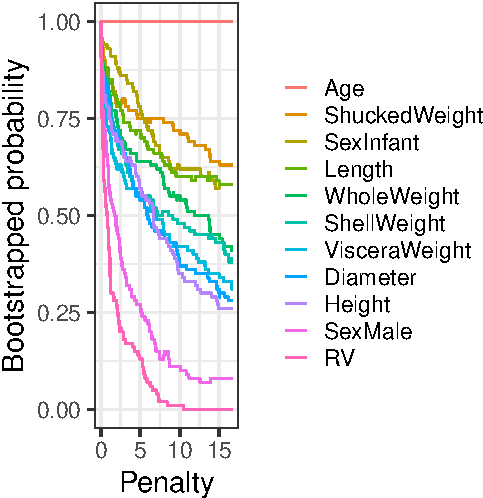
\includegraphics{Executive-summary-Group-Work_files/figure-latex/unnamed-chunk-2-1} \end{center}

We performed an exhaustive search of all models to determine the best
model for each group allowing for different numbers of parameters.
Models using 3 or 4 predictors seemed the best compromise between the
number of predictors and representation across the sexes. Using bglmnet,
we determined bootstrapped selection probabilities for each of the
variables and selected the 3 to 4 most frequently occurring variables
for the model of each group.

\begin{center}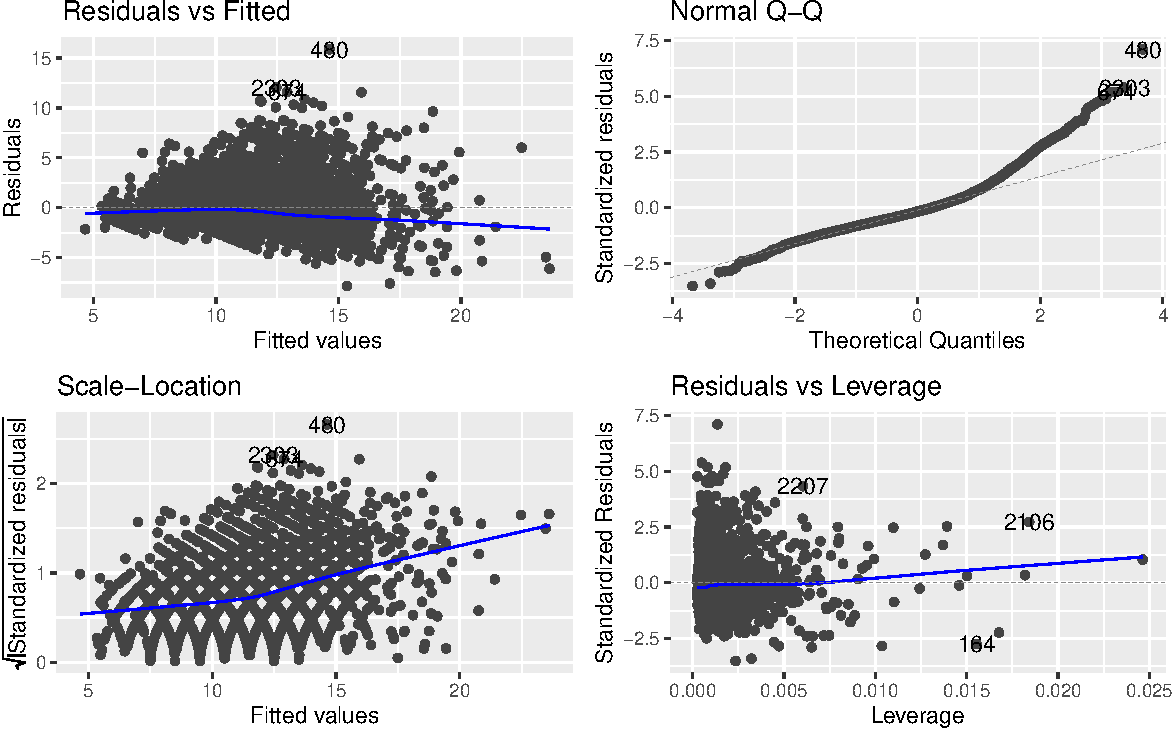
\includegraphics[width=0.8\linewidth]{Executive-summary-Group-Work_files/figure-latex/unnamed-chunk-3-1} \end{center}

Having selected these models, we used diagnostic plots to perform
assumption checking. Linearity, homoscedasticity and normality
assumptions were satisfied, and high-leverage outlier points were
identified and removed. When rerunning the above steps of the
outlier-removed we obtained the same models. To validate the stability
of the models selected, we used mplot with an adaptive fence procedure,
using 80 bootstrap samples over a grid of 100 parameter values.

\begin{center}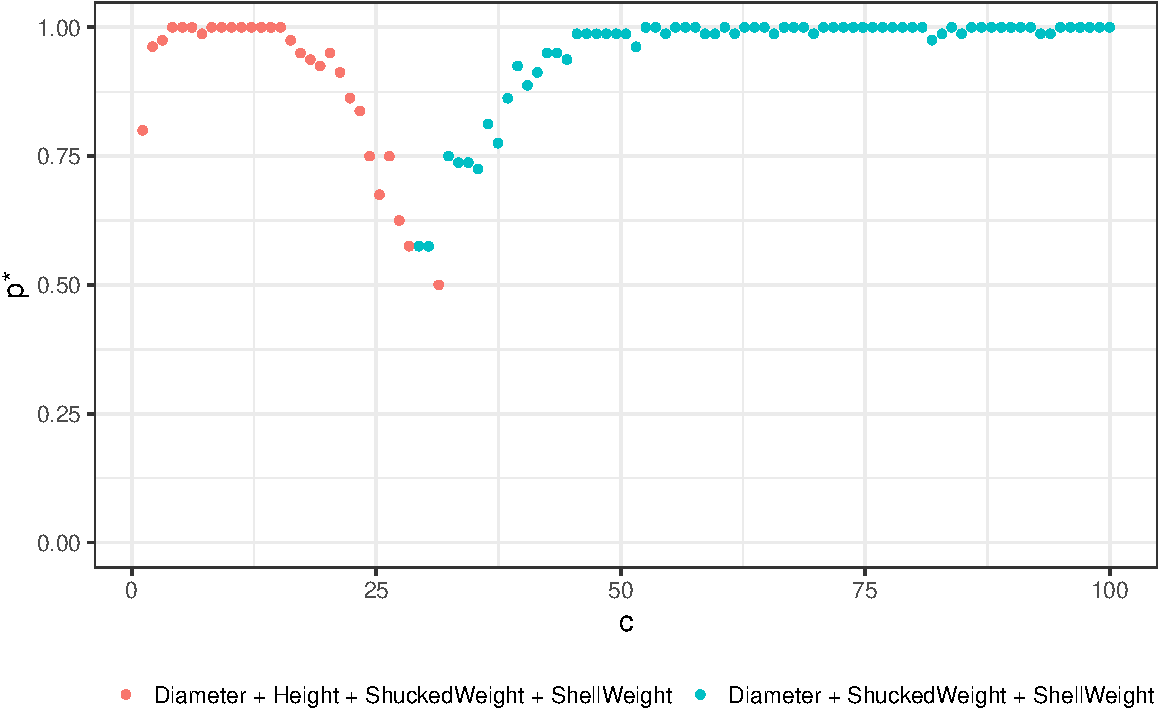
\includegraphics[width=0.8\linewidth]{Executive-summary-Group-Work_files/figure-latex/unnamed-chunk-4-1} \end{center}

\hypertarget{results}{%
\subsection{Results}\label{results}}

The \(R^2\) value for the combined population model is 0.5181,
indicating that around half of the variance in the age variable was
explained by our model. This is likely due to the presence of moderate
amounts of noise in the data.

There is generally little difference in out-of-sample predictive ability
- measured using mean absolute error and mean squared error - between
models for different groups. There is little to no improvement using
models per Sex versus a model ignoring Sex, although it is worth noting
that the model for the infant group performs somewhat better than male
and female. As the balance of sexes in the data is roughly even, this
may be why the overall population model performs similar to, or better
than, individual models for the male and female populations.

\hypertarget{discussion-and-conclusion}{%
\subsection{Discussion and conclusion}\label{discussion-and-conclusion}}

Our analysis of the data is mainly limited by the presence of the noise
in the response variable. Additionally, there appears to be relatively
high variance in the independent variables of diameter, height and
weight within the adult population and low correlation with age, when
compared with the infant population. Infant abalones are still growing,
unlike adult abalones, which may explain why measures of their size are
so much more strongly associated with their age.

All in all, we were able to use mplot to perform an exhaustive search of
models and select a subset of independent variables which produced a
stable model. The model we chose performed reasonably well at predicting
values of the age of an abalone given physical measurements despite the
presence of noise in the dataset.

\hypertarget{r-echo-false-fig.width6.2-fig.height4-out.width80-plotabalone.best2.af-best.only-true-legend.position-bottom}{%
\section{\texorpdfstring{\texttt{\{r\ echo\ =\ FALSE,\ fig.width=6.2,\ fig.height=4,\ out.width="80\%"\}\ \#\ plot(abalone.best2.af,\ best.only\ =\ TRUE,\ legend.position\ =\ "bottom")\ \#}}{\{r echo = FALSE, fig.width=6.2, fig.height=4, out.width="80\%"\} \# plot(abalone.best2.af, best.only = TRUE, legend.position = "bottom") \#}}\label{r-echo-false-fig.width6.2-fig.height4-out.width80-plotabalone.best2.af-best.only-true-legend.position-bottom}}

\hypertarget{r-echo-false-fig.width6-fig.height3-out.extraangle-90-plotabalone.full.vis-which-boot-max.circle-7-seed-1}{%
\section{\texorpdfstring{\texttt{\{r\ echo\ =\ FALSE,\ fig.width=6,\ fig.height=3,\ out.extra=\textquotesingle{}angle=-90\textquotesingle{}\}\ \#\ plot(abalone.full.vis,\ which\ =\ "boot",\ max.circle\ =\ 7,\ seed\ =\ 1)\ \#}}{\{r echo = FALSE, fig.width=6, fig.height=3, out.extra='angle=-90'\} \# plot(abalone.full.vis, which = "boot", max.circle = 7, seed = 1) \#}}\label{r-echo-false-fig.width6-fig.height3-out.extraangle-90-plotabalone.full.vis-which-boot-max.circle-7-seed-1}}

\hypertarget{r-echo-false-fig.width6-fig.height3-out.extraangle-90-plotabalone.full.vis-which-lvk-max.circle-7-seed-1}{%
\section{\texorpdfstring{\texttt{\{r\ echo\ =\ FALSE,\ fig.width=6,\ fig.height=3,\ out.extra=\textquotesingle{}angle=-90\textquotesingle{}\}\ \#\ plot(abalone.full.vis,\ which\ =\ "lvk",\ max.circle\ =\ 7,\ seed\ =\ 1)\ \#}}{\{r echo = FALSE, fig.width=6, fig.height=3, out.extra='angle=-90'\} \# plot(abalone.full.vis, which = "lvk", max.circle = 7, seed = 1) \#}}\label{r-echo-false-fig.width6-fig.height3-out.extraangle-90-plotabalone.full.vis-which-lvk-max.circle-7-seed-1}}

\hypertarget{analysis-1}{%
\subsection{Analysis}\label{analysis-1}}

\hypertarget{results-1}{%
\subsection{Results}\label{results-1}}

\hypertarget{references}{%
\subsection{References}\label{references}}

%\showmatmethods


\bibliography{bibliography}
\bibliographystyle{jss}



\end{document}

